\documentclass{article}
\usepackage[utf8]{inputenc}
\usepackage{mathtools}
\usepackage{amssymb}
\usepackage{graphicx}
\usepackage{listings}
\usepackage{float}
\usepackage{gensymb}
\usepackage{amsthm}
\usepackage{longtable}
\usepackage{adjustbox}
\usepackage{physics}
\usepackage{hyperref}
\usepackage[makeroom]{cancel}

\theoremstyle{definition}
\newtheorem{definition}{Definition}
\newtheorem{proposition}{Proposition}
\newtheorem{example}{Example}

\title{Statistical Field Theory}
\author{quinten tupker}
\date{October 9 2020 - \today}

\begin{document}

\maketitle

\section*{Introduction}

These notes are based on the course lectured by Dr Christopher E Thomas in
Michaelmas 2020. Due to the measures taken in the UK to limit the spread of
Covid-19, these lectures were delivered online. These are not meant to be an
accurate representation of what was lectures. They solely represent a mix of
what I thought was the most important part of the course, mixed in with many
(many) personal remarks, comments and digressions... Of course, any
corrections/comments are appreciated.

Statistical Field Theory is an extension of statistical physics. It assumes one
is familiar with statistical physics, and in particular, focuses on the study on
phase transitions. This course in particular follows David Tong's notes quite
closely.

\section{From Spin to Fields}

So why do we consider fields? Here we look at a model that shows the origin of
this connection.

\subsection{The Ising model}

The Ising model studies a lattice where each point on the lattice is assigned a
spin $S_i = \pm$. Consequently, the energy of the lattice is

$$ E = -B \sum_i S_i - J \sum_{<i, j>} S_i S_j $$

where $B$ is the external magnetic field strength, $J$ is the strength of
neighbour-neighbour interactions and $<i, j>$ is any nearest neighbour pair.
When $J > 0$, states tend to align (ferromagnetic behaviour) whereas if $J < 0$
states will prefer not to align (anti-ferromagnetic behaviour). We will focus on
the $J > 0$ case. But of course, due to heat there some statistical randomness,
and we want to include that. As such, we consider the canonical ensemble with
$\mathbb{P} (S_i) = e^{-\beta E(S_i)} / Z$ where $Z$ is the partition function,
$\beta = 1 / T$, and the Boltzmann constant $k_B = 1$. As ever in statistical
physics, we can derive everything from the partition function. Particularly
important in our case is the Free Energy, $F = \langle E \rangle - TS = -T \ln
(Z)$, and $dF = -S dT - p dV - M dB$ (so we can find S, p and M from F as well).

In statistical physics, we are particularly interested in the equilibrium state
(which occurs at the minimum of the free energy when temperature is constant),
and since we are looking at a magnetic system, we are particularly interested in
the equilibrium magnetisation. This can be calculated as

$$ m = \frac{1}{N} \sum_i \langle S_i \rangle = \frac{1}{N \beta} \partial_B
\ln(Z) $$

Now all that remains is to calculate $Z$ to find $m$. Unfortunately, in
dimension 3 or greater this is impossible (how impossible?), and it is still
hard in lower dimension. Consequently we take a different approach using the
so-called ``effective free energy'', which is defined such that

$$ \sum_m \sum_{\{S_i\} | m} e^{-\beta E[S_i]} = \sum_m e^{-\beta F(m)} $$

where $F(m)$ is the effective free energy. Since we can assume $N$ is large
(around $10^{23}$), we can then write18

$$ Z = N / 2 \int_{-1}^1 dm \, e^{-\beta F(m)}  = N / 2 \int_{-1}^1 dm \,
e^{-\beta N f(m)}$$

where $f(m) = F(m) / N$. From here, we can calculate the equilibrium field by
considering that since $N$ is large, the value contributing the most to the
integral is where $\partial_m f = 0$, and this is how the equilibrium $m$ is
calculated. This approach is called the \textbf{steepest descent approximation},
and we find here that $F_{\text{thermodynamic}} \approx F(m_{\text{min}})$.

This is all very well and nice, but the issue is that we still don't know how to
calculate $F(m)$, and it turns out that this is about as hard as calculating
$Z$. As such, we use the \textbf{mean field approximation}

$$ E \approx -B \sum_i m - J \sum_{<i, j>} m^2 = -BNm - \frac{1}{2} N J q m^2 $$

where $q = 2 \text{dim(space)}$ for a cubic latice in a space dimension dim.
Now,

$$ e^{-\beta N f(m)} = \sum e^{-\beta E(S_i) \approx \Omega(m) e^{-\beta
    E(m)}} $$

so in order to find $f(m)$ we need to know $\Omega(m)$ which is the number of
ways for a given energy state to occur, but since $m$ depends only on the number
of positive and negative spins states, $N_\uparrow, N_\downarrow$, and in
particular $N = N_\uparrow + N_\downarrow$ we see the number of total states is

$$ \ln(\Omega) = \ln \binom{N}{N_\uparrow} \approx N (\ln(2) - \frac{1}{2}(1 +
m) \ln(1 + m) - \frac{1}{2} (1 - m) \ln(1 - m)) $$

by Stirling's approximation. Consequently we find that

$$ f(m) \approx -Bm - \frac{1}{2} J q m^2 - \frac{1}{\beta} (\ln(2) -
\frac{1}{2} (1 + m) \ln(1 + m) - \frac{1}{2} (1 - m) \ln(1 - m)). $$

From here  by taking $\partial_m f = 0$, we find

$$ \beta(B + Jqm) = \frac{1}{2} \ln \left( \frac{1 + m}{1 - m} \right) $$

or equivalently

$$ m = \tanh(\beta (B + Jqm)). $$

From here, we can solve implicitly, but there is another approach we can take,
which is the way we will go about this. Just as a side note, we can see the
reason this is called the mean field approximation here as well: it is as if $m$
just shifts to external field to $B_{\text{eff}} = B + Jqm$. [End of lecture 1.]

\subsection{Landau Theory of Phase Transitions}

The remarkable part about the Ising model described above is not its
correctness. In fact, it is often incorrect, but rather its universality. It can
be applied in a wide variety of situations. As such, Landau tried to develop a
more general theory of phase transitions. Here we work through an extended
example to examine the general features of these. In particular, we study the
behaviour of the equilibrium $m_{\text{min}}$ when various quantities are varied.

From before, we can approximate $f$ for small $m$ as

$$ f(m) \approx \cancel{-\frac{1}{\beta} \ln(2)} - B m + \frac{1}{2} (\frac{1}{\beta} -
Jq) m^2 + \frac{1}{12\beta} m^4 + \dots $$

where we ignore the constant term since it does not affect anything. We start
with the $B = 0$ case where we find that

$$ f(m) = \frac{1}{2} (T - T_c) m^2 + \frac{1}{12} T^4 m^4  $$

where we define the \textbf{critical temperature} to be $Tc = Jq$. Then we get
the following scenarios.

\begin{figure}[H]
  \centering
  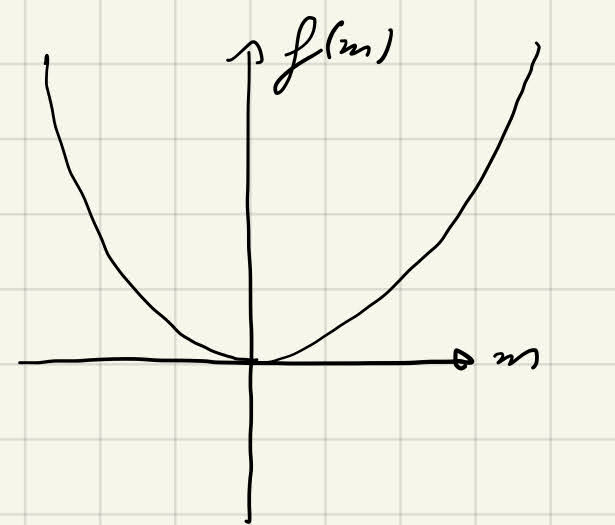
\includegraphics[width=5cm]{res/SFT/f_vs_m_high_T_B0}
  \caption{$T > T_c$}
  \label{figure: f_vs_m_high_T_B0}
\end{figure}

\begin{figure}[H]
  \centering
  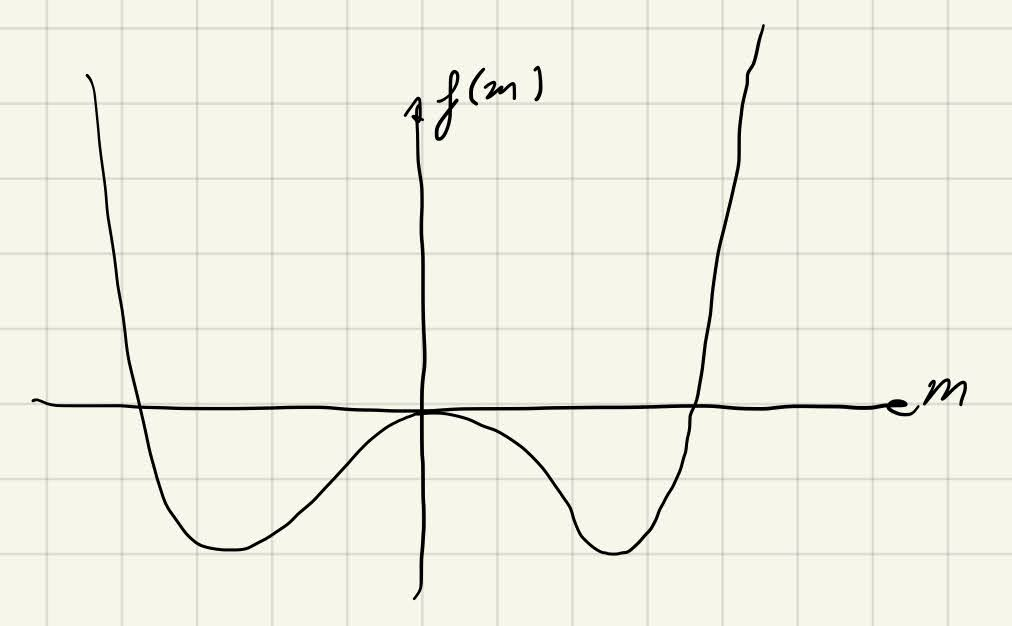
\includegraphics[width=5cm]{res/SFT/f_vs_m_low_T_B0}
  \caption{$T < T_c$}
  \label{figure: f_vs_m_low_T_B0}
\end{figure}

\begin{figure}[H]
  \centering
  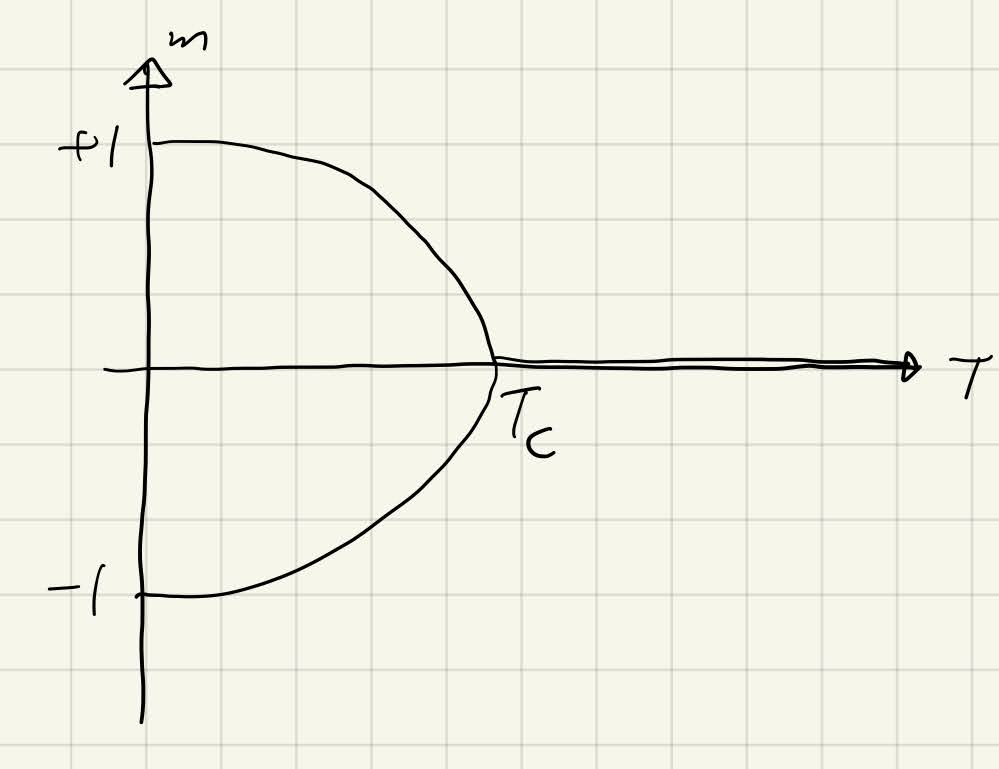
\includegraphics[width=5cm]{res/SFT/m_vs_T_B0}
  \caption{$m_{\text{min}}(T)$ for $B = 0$}
  \label{figure: m_vs_T_B0}
\end{figure}

The middle graph is meant to be symmetric, and we see here that $m_{\text{min}}$
can take two different values

$$ m_{\text{min}} = \pm m_0 = \pm \sqrt{\frac{3(T_c - T}{T}} $$

Now some definitions apply here. This is a \textbf{second order} or
\textbf{continuous} phase transition since $m$ is continuous in the quantity
being varied. $m = 0$ is called the \textbf{disordered phase}, and $m \neq 0$ is
called an \textbf{ordered phase}. \textbf{Spontaneous symmetry breaking} is what
we call the loss of symmetry in $m$ when $T$ decreases below $T_0$ (since $m$ is
forced to choose a positive or negative value). Finally, these terms all extend
to arbitrary \textbf{order parameter} $m$. We finally compute

$$ f(m_{\text{min}}) =
\begin{cases}
  0 & T > T_c \\
  -\frac{3}{4} \frac{(T_c - T)^2}{T} & T < T_c
\end{cases} $$

We can also look at the heat capacity here, and how that various with
temperature. Heat capacity may be defined as

$$ C = \partial_T \langle E \rangle = \beta^2 \partial_\beta^2 \ln(Z) $$

since recall that $\langle E \rangle = -\partial_\beta \ln(Z)$. Using $Z \approx
-\beta N f(m_{\text{min}})$ we find $c = C / N$ has

$$ c =
\begin{cases}
  0 & T \to T_c^+ \\
  3/2 & T \to T_c^-
\end{cases}
$$

so $c$ is a first order phase transition - ie. discontinuous.

The above scenario considered $B \neq 0$, but when $B = 0$ we get a different
situation. In particular, we do not get spontaneous symmetry breaking since the
system is no longer symmetric. In this case, the above graphs are skewed to the
right or the left unevenly leaving global minimum (the ``true'' minimum) and a
so-called \textbf{metastable} state.

Finally, we can observe another discontinuous phase transition when we study
$m_{\text{min}}$ as a function of $B$ at low $T$ ($T < T_c$). Since we're below
the critical temperature, the global minimum does not smoothly slide through 0,
but instead abruptly shifts from negative to postive (or the other way around)
giving a 1st order phase transition. Incidentally, I find this a bit odd, since
this really only makes sense in the 1D case, but as we will see later Mean Field
Theory (MFT) does not work in 1D. But in higher dimensions, $m$ is a vector and
instead of getting two local minima as above, we get a tilted (for $B \neq 0$)
circular valley where $f(m)$ is low. In this case, no phase transition occurs,
since the minimum just smoothly moves around this circular valley as $B$ is
varied...

\begin{figure}[H]
  \centering
  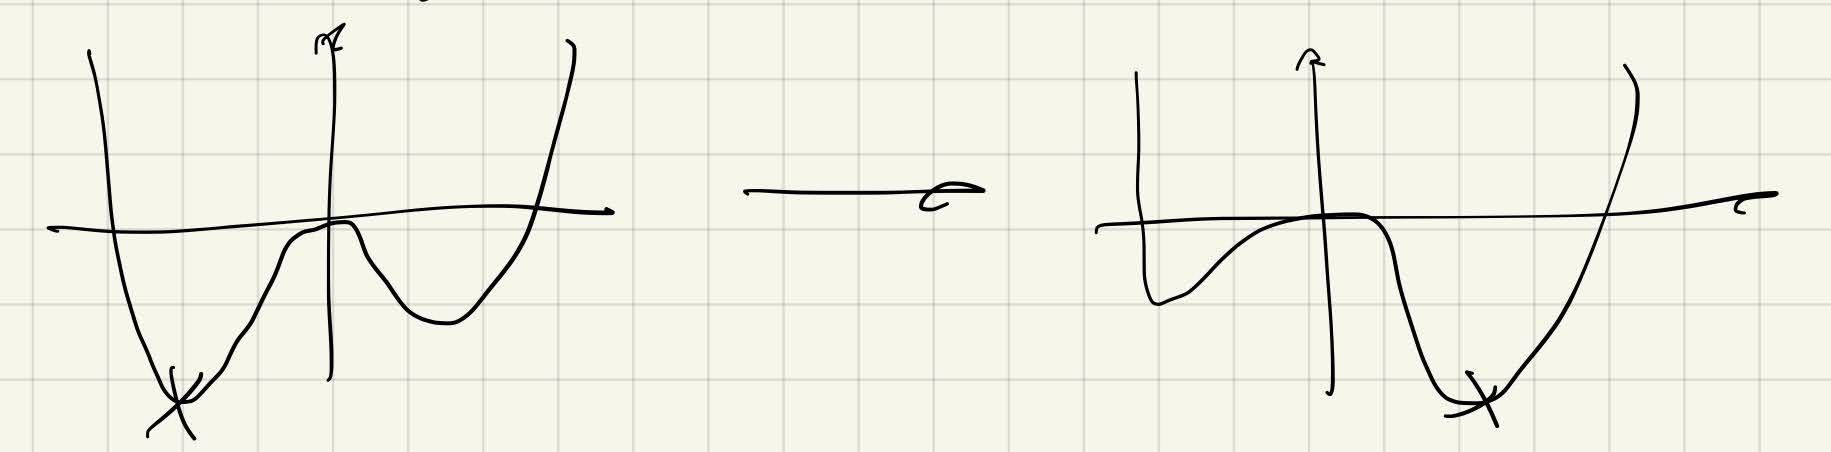
\includegraphics[width=10cm]{res/SFT/m_min_vs_B}
  \caption{$m_{\text{min}}$ vs $B$}
  \label{figure: m_min_vs_B}
\end{figure}

\begin{figure}[H]
  \centering
  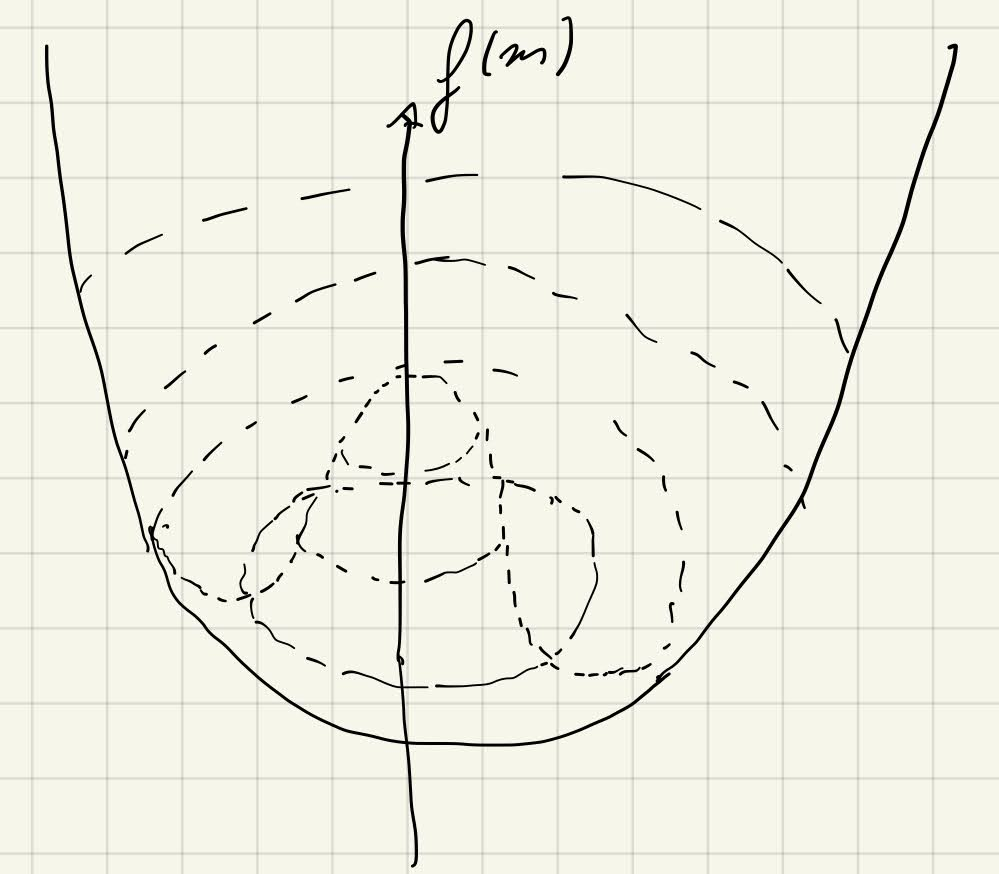
\includegraphics[width=5cm]{res/SFT/f_vs_m_2d}
  \caption{$f(m)$ vs $m$ in 2D}
  \label{figure: f_vs_m_2d}
\end{figure}

Anyways, some other asymptotic behaviour includes that when $T \approx T_c$, we
get

$$ f(m) \approx -Bm + \frac{1}{12} T_c m^4 $$

leaving

$$ m \sim B^{1/3} $$

If we define magnetic susceptibility (the \textbf{response function} in this
context) to be $\chi = \partial_B m|_T$ we see that for $T > T_c$ we have

$$ f(m) \approx -Bm + \frac{1}{2} (T - T_c) m^2 + \dots $$

so

$$ m \approx \frac{B}{T - T_c} $$

so

$$ \chi \sim \frac{1}{T - T_c} $$

and for $T < T_c$

$$ \chi \sim \frac{1}{|T - T_c|} $$

\subsection{The Validity of MFT}

The purpose of all these calculations at the end of the last section is to find
some important set of numbers that we can use to check our theory with in the
real world. In particular, what we looked for were the \textbf{critical
  exponents}, which are

\begin{align*}
  m &\sim (T_c - T)^\beta & \beta &= 1/2 & T &< T_c \\
  c &\sim c_\pm |T - T_c|^{-\alpha} & \alpha &= 0 && \\
  \chi &\sim |T - T_c|^{-\gamma} & \gamma &= 1 && \\
  m &\sim B^{1/\delta} & \delta &= 3 &&
\end{align*}

in our worked example. Now for results, we find that in general, MFT fails
entirely below a certain \textbf{lower critical dimension}, $d_i$ and works correctly
above a certain \textbf{upper critical dimension}, $d_u$. In between it is structurally
accurate (can detect the right phase transitions) but inaccurate (finds the
wrong critical exponents). The Ising fails for dimension 1, gets the right
structure for dimensions 2 and 3, and works for dimension 4 and above. It is, as
expected, closer to the correct value for dimension 3 than for 2, but still can
be quite off.

Nevertheless, as mentioned earlier, the power of the MFT is not in its
correctness, but in its universality. Also, often structure is more important.
After all, if you can predict a phenomenon will happen, you can then carry out
an experiment to measure it more accurately. On the other hand, it is far harder
to use experiment to search for interesting phenomenon without knowing where to
look. So it is still quite powerful. Also, the fact that critical
exponents exist, and that critical points exist is a powerful bit of
universality that MFT gives.

To illustrate its universality, we can consider liquid-gas transitions. Here,
van der Waals analysis is completely off in its critical exponents, although it
does predict the correct type of phenomenon. However in three dimensions, the
Ising model agrees well. How do we implement the Ising model for a gas. Although
it's not at all obvious it will work, the implementation is actually quite
natural. Assume that a space consists of a lattice, and that every lattice is
assigned a value of 1 or 0 based on whether or not it is occupied by a particle.
Also assume that any point on the lattice can be occupied by no more than 1
particle at a time. Then we get

$$ E = -4J \sum_{<i j>} n_i n_j - \mu \sum n_i $$

We can proceed from there as usual. [End of lecture 2]

\subsection{Landau-Ginzburg Theory}

We aim to improve on Landau theory, and somehow the obvious generalisation is to
allow $m$ to vary through space as $m(x)$, but doing so in a way that it is
analytic, so that the calculations involved still stay relatively simple...

Concretely, that means assuming we have a large number of sites $N$, but that
these sites are all grouped into clusters of $N'$ sites, which is still a large
number, but significantly smaller than $N$. Then we define for each cluster, a
centre $x$, and we assign $m(x)$ the value of the average magnetisation of this
cluster. However, since $1 << N' << N$, everything is still analytic, etc. Or so
we assume.

Consequently we can calculate the partition function in much the same way with
the same effective free energy, except now the effective free energy is a
functional instead of a function:

$$ Z = \sum_{m(x)} e^{-\beta F[m(x)]} $$

This can be written as a functional integral (otherwise known as a path integral)

$$ Z = \int Dm[x] e^{-\beta F[m(x)]} $$

and now instead of probabilities we get probabilty density

$$ p(m(x)) = \frac{e^{-\beta F[m(x)]}}{Z}. $$

Now, we have a number of conditions that we require this effective free energy
to satisfy:

\begin{itemize}
\item locality: basically, it takes the form
  $$ F[m(x)] = \int d^dx f[m(x)] $$
  where $f$ depends on $m, \nabla m, \nabla^2 m, \dots$
\item $\mathbb{Z}_2$ symmetry when $B = 0$ under $m \mapsto -m$
\item Analyticity - we assume it has a Taylor expansion
\item we are only interested in $m$ that are slowly varying in space
\end{itemize}

Now, focusing on the $B = 0$ case we see that the effective free energy must
take the form

$$ F[m(x)] = \int dx (\frac{1}{2} \alpha_2(T) m^2 + \frac{1}{4} \alpha_4(T) +
\frac{1}{2} \gamma(T) (\nabla m)^2) $$

where the odd terms are eliminated due to symmetry (of course, when $B \neq 0$
we can add in these odd terms again).

Unfortunately it is hard to find an general way to calculate $\alpha_2,
\alpha_4, \gamma$. but we can say that $\alpha_4, \gamma > 0$ and $\alpha_2$
changes sign at $T_c$/ In particular, in MFT,

$$ \alpha_2 \sim (T - T_c), \alpha_4 \sim \frac{1}{3} T. $$

Just as in plain Landau theory, we use the saddle point approximation that $Z =
\int dm(x) e^{-\beta F(m(x))}$ is focused on the saddle point of $F$, but this
time to find it we need to use the Euler-Lagrange approach, yielding the
equation for the equilibrium:

$$ \gamma \nabla^2 m = \alpha_2m + \alpha_4 m^3 $$

How well does this theory work? We can check that if we assume $m$ is constant,
then we get back to Landau theory, so we know that at the very least, this
theory cannot be worse than Landau theory. As our first development we then look
at the notion of domain walls, and see whether or not those can be of any help.
In particular, we want to see what a solution to the following looks like in the
one dimensional case:

$$ \partial_x^2 m = \alpha_2 m + \alpha_4 m $$ 

where $m = \pm m_0$ as $x \to \pm \infty$. The solution works out to $m = m_0
\tanh(\frac{x - x_0}{W})$ where the width, $W = \sqrt{-\gamma / \alpha_2}$.

This models how the system changes state half-way, and since these don't occur
in ordinary Landau theory. As such, to compare the two it would be helpful to
see what the free energy cost of having a domain wall is. We may calculate this
as

\begin{align*}
  F_W
  &\sim L^{d - 1} \int dx \gamma(\partial_x)^2 \\
  &\sim L^{d - 1} \gamma m_0^2 / W \\
  &= L^{d - 1} \sqrt{-\gamma \alpha_2^3 / \alpha_4^2}
\end{align*}

where $L$ is the ``length'' of the system. Now curiously, this allows us to see
why Landau fails in 1 dimension, but not (as much) in 2 dimensions.

Consider a 1 dimensional space length $L$, starting in state $m_0$ and ending in
some other state, for $T < T_c$, meaning that $\alpha_2 < 0$. We then see that

$$ \mathbb{P}(\text{wall at } x = x_0) = \frac{e^{-\beta F_W}}{Z} $$

$$ \mathbb{P}(\text{wall somewhere}) \sim \frac{L}{W} \frac{e^{-\beta
    F_W}}{Z} $$

meaning that

$$ \mathbb{P}(n \text{ walls}) = e^{-n\beta F_W} / Z \int_0^L dx_1 \int_{x_1}^L
dx_2 \dots \int_{x_{n - 1}}^L dx_n = \frac{1}{Z n!} \left( \frac{L e^{-\beta
      F_W}}{W} \right)^n. $$

Consequently we can calculate the probabilities of how the final state of the
rod ends up:

$$ \mathbb{P}(m \to m_0) = \frac{1}{Z} \cosh \left( \frac{Le^{-\beta F_W}}{W}
\right) $$

$$ \mathbb{P}(m \to -m_0) = \frac{1}{Z} \sinh \left( \frac{Le^{-\beta F_W}}{W}
\right) $$

Now as $L \to \infty$, we see that these probabilities stay about the same,
meaning that the state of the rad stays more or less random. Why does this
argument fail in two dimensions? Well, the calculation does change a bit since
we're in two dimensions, but we also have the fact that $F_W$ may depend on $L$
in this scenario, meaning that in effect, the probabilities above instead
converge to 0 and 1, meaning that a phase transition does indeed occur. [End of
lecture 4]

\subsubsection{Path Integrals}

So how do we evaluate the path integrals we deal with

$$ Z = \int \mathcal{D}m(x) e^{-\beta F[m(x)]} $$

For $B = $ we get the general form

$$ F[m(x)] = \int d^dx (\frac{1}{2} \gamma (\nabla \phi)^2 + \frac{1}{2} \alpha_2
\phi^2 + \alpha_4 \phi^4 + \dots) $$

the path integral can be done when $F$ is at most quadratic in $\phi$. Small
higher order terms are hard, but still feasible, and that's more or less it.
Importantly, for $\alpha_2 = \mu^2$ when $\mu$ is small, this becomes hard to
evaluate since higher order terms do matter. This case will be treated
separately.

Now, to perturb we write $\tilde{\phi} = \phi - \langle \phi \rangle$ and then

$$ F(\tilde{\phi}) = F(m_0) + \frac{1}{2} \int d^dx \gamma (\nabla
\tilde{\phi})^2 + \alpha_2 \tilde{\phi}^2$$

where $\langle  \phi \rangle = \pm m_0$ for $T < T_C$. To start evaluating
things, we use the Fourier space, so $\phi_k = \int d^d x e^{-i k \cdot x}
\phi(x)$ for mommentum $k$. Since we're on a lattice, we take $\phi_k = 0$ for
$k > \lambda = \pi / a$ the UV cut-off. Writing $\phi = \int
\frac{d^dk}{(2\pi)^d} e^{ik \cdot x} \phi_k$, we see that

\begin{align*}
  F(\phi_k) &= \frac{1}{2} \int \frac{d^d k_1}{(2\pi)^d} \frac{d^d k_2}{(2\pi)^d} \int d^d x (-\gamma k_1 \cdot k_2 + \mu^2) \phi_{k_1} \phi_{k_2} e^{i(k_1 + k_2) \cdot x} \\
            &= \frac{1}{2} \int \frac{d^d k}{(2\pi)^d} (-\gamma (-k) \cdot k + \mu^2) \phi_k \phi_{-k} \\
            &= \frac{1}{2} \int \frac{d^d k}{(2\pi)^d} (\gamma k^2 + \mu^2) |\phi_k|^2 \\
            &= \frac{1}{2V} \sum_k (\gamma k^2 + \mu^2) |\phi_k|^2
\end{align*}

Now, we can calculate that the measure in our path integral is

$$ \int \mathcal{D}\phi(x) = \prod_k \left( N \int d\phi_k d\phi_k^* \right) $$

where $N$ is some normalisation constant which we will ignore from hereon since
it does not matter for the calculations we do. Consequently we can claulate

\begin{align*}
  Z &= \prod_k \int  d\phi_k d\phi_k^* e^{-\frac{\beta}{2V} \sum_k (\gamma k^2 + \mu^2) |\phi_k|^2} \\
    &= \prod_k \int d\phi_k d\phi_k^* e^{-\frac{\beta}{2V} (\gamma k^2 + \mu^2) |\phi_k|^2}
\end{align*}

where the last result is just a Gaussian leaving us with

$$ Z = \prod_k \sqrt{\frac{2\pi V T}{\gamma k^2 + \mu^2}} $$

Relating this to $F_{therm}$ via $Z = e^{-\beta F_{therm}}$ we find that

$$ F_therm / V = - \frac{T}{2V} \sum_k \ln \left( \frac{2\pi V T}{\gamma k^2 +
    \mu^2} \right) = \frac{-T}{2} \int \frac{d^dk}{(2\pi)^d} \ln \left(
  \frac{2\pi V T}{\gamma k^2 + \mu^2} \right) $$

which might look like it diverges. This is the one place where the normalisation
constant $N$ does matter, and does fix the issue. Regardless, we continue to
ignore it.

\begin{example}
  Compute $c = C/V$.
  \begin{align*}
    C &= \frac{\beta^2}{V} \partial_\beta^2 \ln(Z) \\
      &= \frac{1}{2} (T^2 \partial_T^2 + 2T \partial_T) \int \frac{d^d k}{(2\pi)^d} \ln \left( \frac{2 \pi V T}{\gamma k^2 + \mu^2} \right) \\
      &= \frac{1}{2} \int \frac{d^d k}{(2\pi)^d} (1 - \frac{2T}{\gamma k^2 + \mu^2} + \frac{T^2}{(\gamma k^2 + \mu^2)^2 })
  \end{align*}
  Here we see that this depends on $d$ quite strongly and the convergence as
  $\Lambda \to \infty$ and we also only care about $k^2$ not $\hat{k}$.
  For the two non-constant terms we see that
  $$
  \int^\Lambda_0 dk \frac{k^{d - 1}}{\gamma k^2 + \mu^2} \sim
  \begin{cases}
    \Lambda^{d - 2} + \dots & d > 2 \\
    \ln(\Lambda) + \dots & d = 2 \\
    \mu^{-1} + \dots & d = 1
  \end{cases}
  $$
  $$
  \int^\Lambda_0 dk \frac{d^d k}{\gamma k^2 + \mu^2} \sim
  \begin{cases}
    \Lambda^{d - 4} + \dots & d > 4 \\
    \ln(\Lambda) + \dots & d = 4 \\
    \mu^{d - 4} + \dots & d < 4
  \end{cases}
  $$
  Consequently, we see that for $d \geq 4$, $c$ is independent of $T$ whereas
  for $d < 4$, $c \sim \mu^{d - 4} \sim |T - T_c|^{-\alpha} \implies \alpha = 2
  - d / 2$. Do remember that we cannot use this calculation near the critical
  point, since the $\phi^4$ term matters there. [End of lecture 2.1]
\end{example}

In general, this approach can help us refine our critical exponent calcuations.
Firstly, note that

$$ \langle \phi(x) \rangle =
\begin{cases}
  0 & T > T_c \\
  \pm m & T < T_c
\end{cases}
$$

Here we define the \textbf{correlation} to be

$$ \langle \phi(x) \phi(y) \rangle> $$

and the \textbf{connected correlation} to be

$$ \langle \phi(x) \phi(y) \rangle_c = \langle \phi(x) \phi(y) \rangle - \langle
\phi \rangle^2 $$

We will see that we are often less interested in the correlation itself, but
more in the length scales on which it is significant. Now to see how we might
examine correlatoins, we consider free energy

$$ F = \int d^d x \langle \frac{1}{2} \gamma (\nabla \phi)^2 + \frac{1}{2} \mu^2
\phi^2 - B(x) \phi(x) \rangle $$

with $Z(B(x)) = \int \mathcal{D}\phi e^{-\beta F}$ as usual. As usual, the
partition function contains a lot of information

\begin{example}
  $$ \frac{1}{\beta} \frac{\delta \ln(Z)}{\delta B(x)} = \frac{1}{\beta^2}
  \frac{\delta Z}{\delta B(x)} = - \langle \phi \rangle_B $$
  which is minus the expected value of $\phi$ for $B = B(x)$.
\end{example}

\begin{example}
  Similarly,
  \begin{align*}
    \frac{1}{\beta^2} \frac{\delta^2 \ln(Z)}{\delta B(x) \delta B(y)}
    &= \frac{1}{\beta^2 Z} \frac{\delta^2 Z}{\delta B(x) \delta B(y)} - \frac{1}{\beta^2 Z^2} \frac{\delta Z}{\delta B(x)} \frac{\delta Z}{\delta B(y)} \\
    &= \langle \phi(x) \phi(y) \rangle_B - \langle \phi(x) \rangle_B \langle \phi(y) \rangle_B
  \end{align*}
  leaving
  $$ \langle \phi(x) \phi(y) \rangle_c = \frac{1}{\beta^2} \frac{\delta^2
    \ln(Z)}{\delta B(x) \delta B(y)} |_{B=0} $$
\end{example}

All we need to do to make use of these nice properties is actually calculating
$Z(B(x))$. We use the same approach as we used earlier for $B = 0$, which is to
use the Fourier space, but now also with Fourier modes $B_k$ of $B$.

$$ F(\phi_k) = \int \frac{d^d k}{(2\pi)^d} \left( \frac{1}{2}(\gamma k^2 +
  \mu^2) \phi_k \phi_{-k} - B_{-k} \phi_k \right) $$

using Gaussian integrals with $\hat{\phi}_k = \phi_k - \frac{Bk}{\gamma k^2 +
  \mu^2}$ we get

$$ F(\hat{phi}_k) = \int \frac{d^d k}{(2\pi)^d} \left( \frac{1}{2} (\gamma k^2 +
  \mu^2) |\hat{\phi}_k |^2 - \frac{1}{2} \frac{|B_k|^2}{\gamma k^2 + \mu^2}
\right) $$

meaning that

\begin{align*}
  Z(B(x)) &= \prod_k \int d \hat{\phi}_k d \hat{\phi}_k^* e^{-\beta F(\phi)} \\
          &= e^{-\beta F_{thermo}} e^{\frac{\beta}{2} \int \frac{d^d k}{(2\pi)^d} \frac{|B_k|^2}{\gamma k^2 + \mu^2}} \\
          &= e^{-\beta F_{thermo}} e^{\frac{\beta}{2} \int d^d x d^d y B(x) G(x - y) B(y)}
\end{align*}

(we split off the parts depending on $B$) where

$$ G(x) = \int \frac{d^d k}{(2 \pi)^d} \frac{e^{-ik \cdot (x - y)}}{\gamma k^2 +
  \mu^2} $$

We then see, from our earlier example, that

$$ \langle \phi(x) \phi(y) \rangle_c = \frac{1}{\beta} G(x - y) $$

We then define the \textbf{correlation length} to be $\xi^2 = \gamma / \mu^2$,
which from our expression for the connected correlation we can see that this is
strongly related the length scale the meaningful correlation occurs on. In
particular, we see that

$$ G(x) = G(|x|) = \frac{1}{\gamma} \int \frac{d^d x}{(2\pi)^d} \frac{e^{-i k
    \cdot x}}{k^2 + 1 / \xi^2} $$

A such (see example sheet 2) we see that

$$ G(r) \sim
\begin{cases}
  \frac{1}{r^{d - 2}} & r << \xi \\
  \frac{e^{-r / \xi}}{r^{(d - 1) / 2}} & r >> \xi
\end{cases}
$$

A such, we see that meaningful fluctation sizes occur for lengths $ r < \xi$ as
we'd hoped. In particular, we see that near the critical point ($\mu^2 \sim |T -
T_c \implies \xi \to \infty$ as $T \to T_c$) meaningful fluctuations occur on
all length scales. Let's try to understand what happens here. In particular,
let's define two \textbf{new critical exponents} (yay!)

$$ \xi \sim |T - T_c|^{-\nu}, \nu = 1/2 $$

$$ \langle \phi(x) \phi(y) \rangle \sim \frac{1}{r^{d -2 + \eta}}, \eta = 0 $$

These values turn out to be correct for $d \geq 4$, but wrong for $d < 4$,
leaving another mystery. Nevertheless, the upper critical dimension seems to fit
with our pattern. To think a bit more about the upper critical dimension notice
that MFT is not obviously wrong if $\langle \phi^2 \rangle < \langle \phi
\rangle^2$. As such we find it useful to define

$$ R = \frac{\int^\xi_0 d^d x \langle \phi(x) \phi(0) \rangle}{\int^\xi_0 d^d x
  m_0^2} $$

where $\langle \phi \rangle = \pm m_0$ for $T < T_c$. Here $R$ is roughly
indicative of the size of the fluctuations we see. In particular, we notice that

$$ R \sim \frac{1}{m_0^2 \xi^d} \int^\xi_0 dr \frac{r^{d - 1}}{r^{d - 2}} \sim
\frac{\xi^{2 - d}}{m_0^2} $$

so from our critical exponents

$$ R \sim |T - T_c|^{(d - 4) / 2} $$

In particular, we see that $d < 4 \implies R \to \infty$ as $T \to T_c$ so MFT
is certainly wrong.

So we can see information about the upper critical dimension using this
approach, but let's see if we can get a bit of a better picture on the
fluctuations as well. [End of lecture 2.2]

\section{Renormalisation}

Here we use the more famous technique of renormalisation. First note that we
treat renormalisation in general, meaning that now

$$ F(\phi) = \int d^d x \left( \frac{1}{2} (\nabla \phi)^2 + \frac{1}{2} \mu^2
  \phi^2 + g\phi^4 + \dots \right) $$

where all we require is that

\begin{itemize}
\item $F$ is analytic about $\phi = 0$
\item $F$ is even, so the same for $\phi \mapsto -\phi$
\item We conventially set the coefficient in front of $(\nabla \phi)^2$ to be
  $\frac{1}{2}$ which is really the same as a rescaling up to units so has no
  effect.
\end{itemize}

We thus get an infinite list of constants $g_n$ to describe our theory, and in
particular, when we renormalise we study how we ``move between theories''. We in
a sense, establish a way to travel between theories and a way to check if two
theories are close enough. This is particularly insightful, as it allows us to
see why universality exists, which naturally arises from many theories being
close to each other in some sense, and we can also clearly see when it breaks
down. As such, we refer to the coefficients $g_n$ as corresponding to a point in
\textbf{theory space}. 

So how do we establish the ``closeness'' of theories? Probably you could build
some kind of metric and that certainly would be interesting on its own. However,
now instead of using a metric, we look at the convergence of theories. In
particular, we notice that since we always approximate theories when we study
them, we really only care about theories ``up to approximation'' or we only care
about them up to the point that they approximate the same thing. In particular,
rescaling shouldn't change the nature of the theory, but it may change the
constants, and seeing which theories converge to the same type when we rescale
is how we determine which theories are close to one another. That is what
renormalisation is. The rescaling of theories, and analysis of their convergence
under this rescaling.

When we rescale, we need to remember that we are almost always using a UV cutoff
$\Lambda \sim 1/a$ for spacing $a$ allowing us to ignore $\phi_k$ for $k >> 1 /
L$ when we are working on length scale $L$. As such, when we rescale by $\zeta >
1$ we also need to rescale the cutoff to $\Lambda' = \Lambda / \zeta$. We then
also split

$$ \phi_k = \phi_k^- + \phi_k^+ $$

where

$$ \phi_k^- =
\begin{cases}
  \phi_k & |k| < \Lambda' \\
  0 & |k| > \Lambda'
\end{cases}
$$

and similar for $\phi_k^+$ (so we want to ignore $\phi_k^+$). We then write

$$ F(\phi_k) = F_0(\phi_k^-) + F_0(\phi_k^+) + F_I(\phi_k^-, \phi_k^+) $$

where $F_I$ is the interaction term. We then write

\begin{align*}
  Z &= \int \prod_{k < \Lambda} d\phi_k e^{-F(\phi_k)} \\
    &= \int \prod_{k < \Lambda'} d\phi_k^- e^{-F_0(\phi_k^-)} \int \prod_{\Lambda' < k < \Lambda} d \phi_k^+ e^{-F_0(\phi_k^+)} e^{-F_I(\phi_k^-, \phi_k^+)} \\
    &= \int \prod_{k < \Lambda'} d\phi_k^- e^{-F'(\phi_k^-)}
\end{align*}

for \textbf{Wilsonian effective free energy} $F'$ (we need to reformat the
theory into one with a UV cutoff after all). The Wilsonian effective free energy
takes the form, again,

$$ F'(\phi) = \int d^dx \left( \frac{1}{2} \gamma' (\nabla \phi)^2 + \frac{1}{2}
\mu'^2 \phi^2 + g'\phi^4 + \dots \right) $$

[so I guess renormalisation is more of a rescaling of the cutoff, and examining
how the theory varies under different cutoffs - makes sense]. Continuing to
reformat things, we set $k' = \zeta k, x' = x / \zeta$ (want to preserve $k
\cdot x$) and rescale the field as $\phi'_k = \sqrt{\gamma'} \phi_j^-$ to get

$$ F'(\phi') = \int d^d x' \left( \frac{1}{2} (\nabla' \phi')^2 + \frac{1}{2}
  \mu^2(\zeta) \phi^2 + g(\zeta) \phi^4 \right) $$

In short then, renormalisation corresponds today

\begin{enumerate}
\item Integrate out modes $\Lambda / \zeta < k < \Lambda$ for $\zeta > 1$
\item rescale $k' = \zeta k$
\item rescale fields to get $1/2$ gradient coefficient [End of lecture 3.0]
\end{enumerate}

So what kind of behaviour can we see when we renormalise a theory? Basically, we
can diverge to $\infty$, approach a fixed point, we can end up in a fixed cycle
or we can wander around aimlessly. Of these, the last two are ``uncommon,'' so
we will focus on the first two. In particular, fixed points of $\xi$ are of
note, since if $\xi' = \xi / \zeta$ then either $\xi = 0$ or $\xi = \infty$. In
the first case, then for $T$ small we get an ordered phase, and $T$ big we get a
disordered phase. This is not so interesting. The interesting case here is $\xi
= \infty$ so we get global behaviour, which is interesting (see examples at
\href{http://physics.weber.edu/thermal/computer.html}{here}).

For flows near a fixed point we use the following terms:

\begin{itemize}
\item a flow is \textbf{irrelevant} if it flows back to the fixed point.
\item a flow is \textbf{relevant} if it flows away from the fixed point.
\item a flow is \textbf{marginal} if it moves somewhere else within an overall
  ``fixed hyperplane''
\end{itemize}

Usually you get an infinite number of irrelevant directions and a finite number
of relevant directions around a fixed point. This is what leads to the
universality that we generally observe. This universality makes the low energy
regime easier to understand, but makes it harder to extrapolate to high energy
physics, since many high energy theories lead to the same low energy physics.
[End of lecture 3.1]

\subsection{Understanding Critical Exponents}

We can use renormalisation to improve our understanding of critical exponents.
To start with we see that at a fixed point there is no sense of scale (?) so we
can write

$$ \langle \phi(x) \phi(0) \rangle = \frac{1}{r^{d - 2 + \eta}} $$

(any other functional would need a sense of scale on dimensional grounds).
Dimensional analysis tells us that $[x] = 1 \implies [\partial_x] = 1$ so in
particular, $[F] = 0, [d^dx] = -d, [\nabla] = 1,$ so $[\phi] = \frac{d - 2}{2}$,
so $\eta = 0$ as before. This disagrees with experiment despite our analysis
being as simple as dimensional analysis. This is because there is a ``hidden
scale'' that comes from the energy cut-off $a$ and so instead we get

$$ \langle \phi(x) \phi(y) \rangle \sim \frac{a^\eta}{r^{d - 2 + \eta}} $$

which gives us a slightly modified dimensional analysis. In particular, if we
rescale $x \mapsto x / \zeta$, so $\phi(x) \mapsto \phi'(x') =
\zeta^{\Delta_\phi} \phi(x)$ with scaling dimension $\Delta_\phi$ leaving

$$ \langle \phi(x) \phi(y) \rangle \sim \frac{1}{r^{d - 2 + \eta}} $$

giving

$$ \Delta_\phi = \frac{d - 2 + \eta}{2}$$ with so-called \textbf{anomolous
  dimension} $\eta / 2$. Consequently, if $t = |T - T_c| / T_c$ then

$$ \xi \sim t^{-\nu} $$

has $\xi \sim 1/\mu \sim 1 / t^{1/2}$ which does not agree with experiment, but
if $[\xi] = -1$ then $t \mapsto \zeta t^{\Delta_t} t$ where $\Delta_t = 1 /
\nu$.

Now, if $\xi$ is the only length scale in our theory, then all other critical
exponents follow from $\eta, \nu$. We work this out now.

\begin{enumerate}
  \item Note that $F_{thermo} = \int d^d x f(t) \implies f \sim t^{d\nu}$. Also,
    $c = \partial_t^2 f \sim t^{d\nu - 2} \sim t^{-\alpha} \implies \alpha = 2 -
    d\nu$. This is known as the \textbf{hyperscaling relation}.
  \item $m \sim \phi \sim t^\beta$ and $\Delta_\phi = \beta \Delta_t \implies
    \beta = \nu \Delta_\phi = \nu (d - 2 + \eta) / 2$
  \item $F \sim \int d^d x B\phi \implies \Delta_\phi + \Delta_B = d \implies
    \Delta_B = (d + 2 - \eta) / 2 \implies \gamma = \nu(2 + \eta)$. This is
    known as \textbf{Fisher's identity}.
  \item We also see that $\delta = \Delta_B / \Delta_\phi = (d + 2 - \eta) / (d
    - 2 + \eta)$.
\end{enumerate}

This works well for the $d=2, 3$ Ising model and for MFT with $d = 4$. However,
it fails for MFT $d > 4$ for $\beta, \delta$ because the $g \phi^4$ term means
we get $m \sim \sqrt{t / g}$. 

Finally, we note that we can characterise interactions by how they scale with
$F(\phi) \sim \int d^d x g_O O(x)$ for some interaction order $O(x)$ where $O(x)
\mapsto \zeta^{\Delta_O} O(x)$ and $\Delta_{g_O} = d - \Delta_O \implies g_O
\mapsto \zeta^{d - \Delta_O} g_O$. Note however that not all interactions take
this form. Just as with renormalisation flows, we can classify these
interactions as \textbf{relevant} for $\Delta_O < d$, \textbf{irrelevant} for
$\Delta_O > d$ and marginal for $\Delta_O = d$. [End of lecture 3.2]

\subsection{Gaussian Case}

There is one case where it is relatively easy to work out renormalisation
explicitly, which is the so-called \textbf{Gaussian case} when

$$ F_0(\phi) = \int d^d x \left( \frac{1}{2}(\nabla \phi)^2 + \frac{1}{2}
  \mu_0^2 \phi^2 \right) = \int^\Delta \frac{d^d x}{(2\pi)^d} \frac{1}{2}(k^2 +
\mu_0^2) \phi_k \phi_{-k} $$

This case is special because here there is no interaction term:

$$ F_0(\phi)= = F_0(\phi^-) + F_0(\phi^+) $$

so

$$ e^{-F'_0(\phi')} = \left( \int \mathcal{D}\phi^+ e^{-F_0(\phi^+)} \right)
e^{-F_0(\phi^-)} = Ne^{-F_0(\phi^-)} $$

So setting $k' = \zeta k, \phi_k = \zeta^{-w} \phi_k$ where $w$ is undetermined
leaves us with

$$ F_0(\phi^-) = \int^{\Delta / \zeta} \frac{d^d k}{(2\pi)^k} \frac{1}{2} (k^2 +
\mu_0^2) \phi_k^- \phi_{-k}^- = \int^\Delta \frac{d^d k'}{(2\pi)^d} \frac{1}{2
  \zeta^d} \left( \frac{k'^2}{\zeta^2} + \mu_0^2 \right) \zeta^{2w} \phi'_{k'}
\phi'_{-k'} $$

so picking $w = (d + 2) / 2$ gives us the right $1/2$ coefficient. Relabelling
$k'$ as $k$ we get our desired result:

$$ F'_0(\phi') = \int^\Delta \frac{d^d k}{(2\pi)^d} \frac{1}{2} (k^2 +
\mu^2(\zeta)) \phi'_k \phi'_{-k} $$

where $\mu^2(\zeta) = \zeta^2 \mu_0^2$ so as mentioned before, for $\xi = 1 /
\mu$,  $\partial_\xi \mu^2 = 0 \implies \mu^2 = \infty$ at $T = \infty$ (so
ignore this case) or $\mu^2 = 0$ (which is the Gaussian fixed point).

As $\mu^2 \phi^2$ gets bigger this becomes the relevant operator. On other hand,
$\alpha_2 (\nabla^2 \phi)^2$ scales as $\alpha_2(\zeta) = \zeta^{-2}\alpha_0$ so
this term is irrelevant. In the more general terms

$$ F(\phi) = \int d^dx \left( \frac{1}{2} (\nabla \phi)^2 + \frac{1}{2} \mu_0^2
  \phi^2 + \sum_4^\infty g_{0n} \phi^n \right) $$

where the $n$s are all even, we get non-trivial interactions terms leading today

$$ g_{0n} \mapsto g_n' + g_{0n} + \delta g_n $$

where $\delta g_n$ arises from the interactions. $\phi'(x') =
\zeta^{\Delta_\phi} \phi(x)$ then means that

$$ F(\phi') = \int d^d x' \zeta^d \left( \frac{1}{2} \zeta^{-2 - 2 \Delta_\phi}
  (\nabla' \phi')^2 + \frac{1}{2} \mu_0^2 \zeta^{-2\Delta_\phi} \phi'^2 +
  \sum_4^\infty g_{0n} \zeta^{-n\Delta_\phi} \phi'^n \right) $$

wher $\Delta_\phi = (d - 2) / 2$ again. The same approach with dimensional
results allows us to return to the original form of the free energy with new
coefficients

$$ g_n(\zeta) = \zeta^{d -n\Delta_\phi} g_{0n} = \zeta^{n + d(1 - n/2)}
g_{0n} $$

\begin{example}
  For the quartic term we find $g_4(\zeta) = \zeta^{4 - d}g_{0n}$ which becomes
  irrelevant for $d > 4$, but relevant for $d < 4$ and marginal for $d = 4$.
  This agrees nicely with what we've found before. For $d > 4$, the quartic term
  ``auto-tunes'' whereas for lower dimension, an experimentalist would have to
  forcibly control it, to prevent it from ``veering off'' whereas for lower
  dimension, an experimentalist would have to forcibly control it, to prevent it
  from ``veering off.'' The problem we find is that for $n > 4$ and $n$ even,
  all $g_n$ are always relevant (except perhaps $d = 1$ for $g_6$?).
\end{example}

Now, as a matter of language, we now will usually use the term MFT or
\textbf{mean field theory} to refer to the Gaussian case specifically, even
though things have changed quite a bit.

Just as a final warning, we'd like to point out the concept of \textit{dangerous
irrelevant terms}. A specific example is the quartic term in the critical
exponents for MFT with $d > 4$. In this case, for $\beta, \delta$ our more basic
analysis fails, but once we include $g_4$ we find that $m_0 \sim (t /
g_4)^\beta$ for $\beta = 1/2$, Here, $\Delta_{g_4} = 4 - d$ gives us
$\Delta_\phi = \beta(\Delta_t - \Delta_{g_4}) = \beta (d - 2)$ and now $\beta =
1/2$ is fully compatible with scaling (so MFT and the scaling approach agree).

All this is just to point out that sometimes, irrelevant terms can change
critical exponeents even though they are ``irrelevant'' in another sense.

\end{document}